\section{Análisis de sensibilidad}
\label{section:sensLambda}

En las secciones anteriores se estudió la respuesta EM de una monocapa desordenada de NPs esféricas e idénticas, soportada por un sustrato que simula a un vidrio BK7 e inmersas en un medio acuoso. Cuando las NPs se iluminan en un configuración ATR, se observa un modo colectivo el cual puede sintonizarse al seleccionar el radio $a$ de las NPs, la fracción de cubierta $\Theta$ de la monocapa y el material de las NPs. En la Fig. \ref{fig:RT-AuAg} se muestran los resultados de la reflectancia de la monocapa de NPs de oro y la de NPs de plata, con los parámetros escogidos aptos para el biosensado. Para esto se buscó que el modo colectivo se excitara dentro del espectro visible, que la reflectancia a las longitudes de onda del modo colectivo sea mínima para un ángulo de incidencia menor a $80^\circ$ y que el ancho del modo colectivo sea el menor posible.

Los biosensores plasmónicos miden cambios en el índice de refracción y su rendimiento puede expresarse mediante la sensibilidad de bulto $S_B$ \cite{estevez2014trends,svedendahl2009refractometric}, que es la dependencia del corrimiento al rojo $\Delta \lambda$ de la excitación ante cambios en el índice de refracción de la matriz $\Delta n_m$, es decir
	\begin{equation}
	S_B = \frac{\Delta \lambda}{\Delta n_m}.
	\end{equation}
Otro parámetro que caracteriza el rendimiento del biosensado es el FWHM $\Gamma$, por lo que se combina éste junto con la sensibilidad de bulto $S_B$, construyendo así la \emph{figura de mérito} (Figure of Merit, $FOM_B$) dada por la expresión
	\begin{equation}
	FOM_B = \frac{1}{\Gamma}\frac{\Delta \lambda}{\Delta n_m}.
	\end{equation}
El empleo de la $FOM_B$ permite comparar no sólo la sensibilidad del biosensor, sino también la desviación del modo, además, de ser un parámetro que permite calificar la calidad de biosensores ópticos con diferentes estructuras \cite{svedendahl2009refractometric}, como puede ser la comparación entre sensores comerciales, basados en el plasmón-polaritón de superficie (Surface Plasmon Polariton, SPP), el modo colectivo observado en los cálculos de la reflectancia bajo el formalismo del CSM y los sensores basados tanto en las PSLR observado en \cite{kabashin2009plasmonic,danilov2018ultra} y en las resonancias de superfice localizadas (Localized Surfaces Plasmon Resonance, LSPR) como las estudiadas en \cite{svedendahl2009refractometric}.




	\begin{figure}[h!]\centering\hspace*{-1.5em}
	\begin{subfigure}{.01\linewidth}\caption{}\label{sfig:SensThetai}\vspace{11cm}\end{subfigure}
	\begin{subfigure}{.95\linewidth}\hspace*{-1em}
	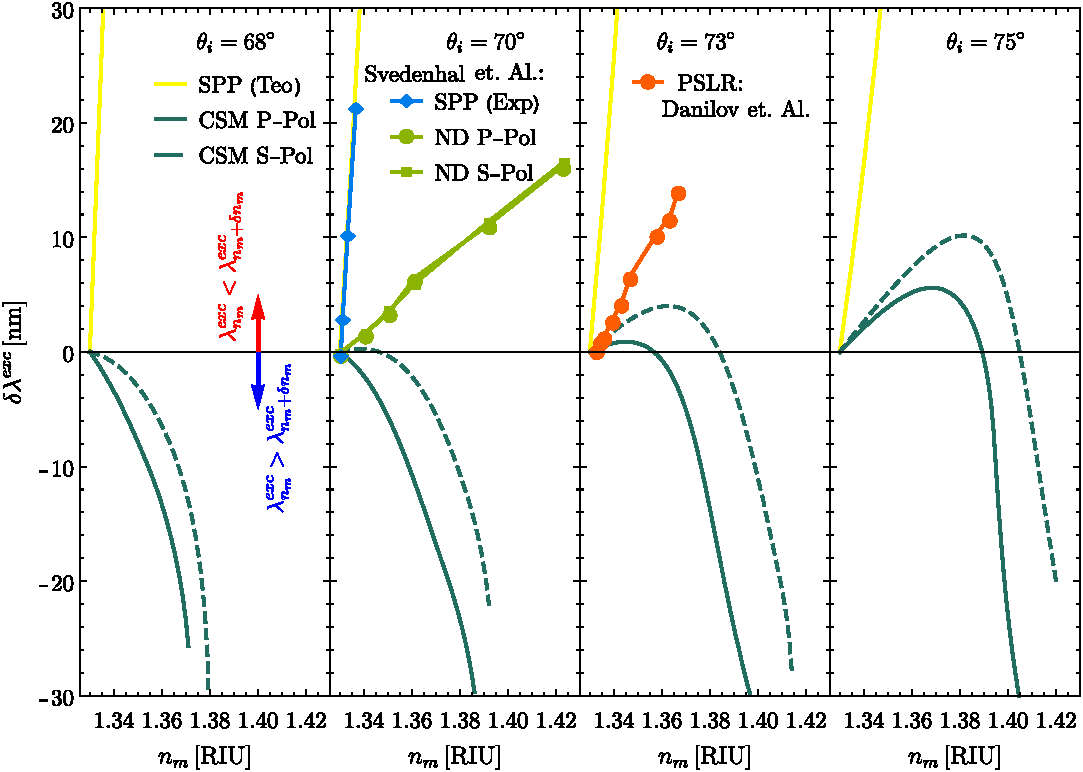
\includegraphics[width=\linewidth]{2-Resultados/figs/11-SPPCSM/1-comparacion_Au.pdf}
	\end{subfigure}\\ \hspace*{-1.5em}
	\begin{subfigure}{.01\linewidth}\caption{}\label{sfig:SensRpRs}\vspace{6.5cm}\end{subfigure}
	\begin{subfigure}{.95\linewidth}\hspace*{-1em}
	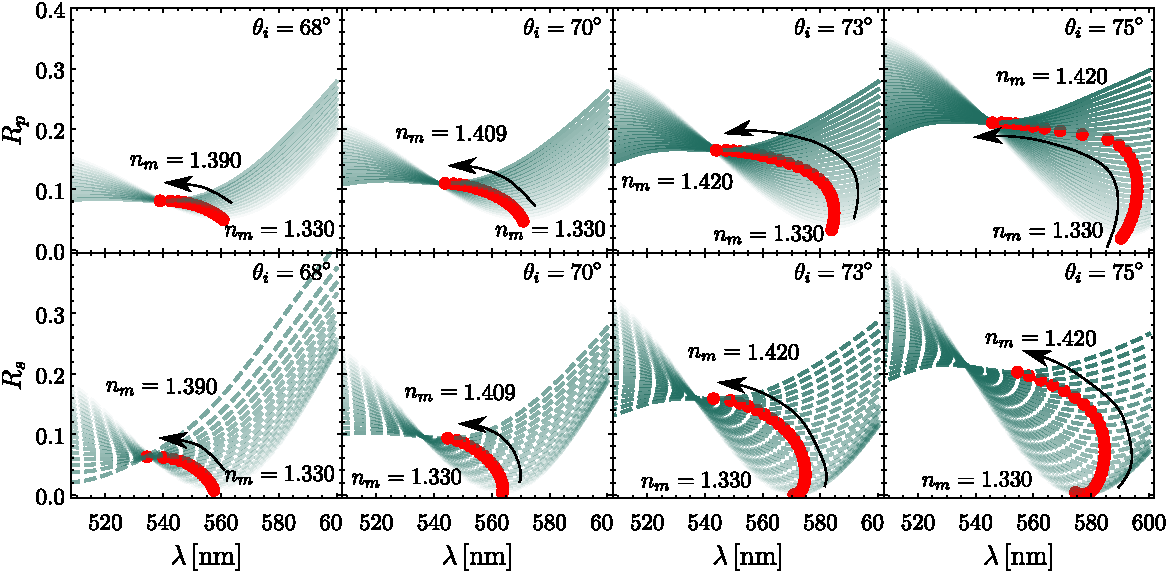
\includegraphics[width=\linewidth]{2-Resultados/figs/11-SPPCSM/2-RpRs}
	\end{subfigure}\vspace*{-.7em}
	\caption{ Comparación de la función dieléctrica como función de la energía $\hbar\omega$ para \textbf{a)} el   oro y \textbf{b)} la plata en bulto (líneas continuas) y para NPs esféricas de radio $a=5$ nm (líneas discontinuas), $a=10$ nm (líneas punteadas) y $a=50$ nm (líneas punto punteadas). La dependencia de la función dieléctrica con la longitud de onda $\lambda$ se muestra en la escala superior.}\label{fig:FinalResults}
	\end{figure}	


Con la finalidad de comparar \ref{fig:SPPCSM} se muestran los cálculos de la reflectancia en configuración ATR para una placa delgada de oro y una de plata ---donde se observa el SPP---, ambas de grosor $d=45$ nm, y para una monocapa de NPs esféricas de oro (con $a=30$ nm y $\Theta=0.125$) y una de NPs de plata (con $a=40$ nm y $\Theta=0.1$) ---donde se observa el modo colectivo---; en todos los casos se tiene un sustrato con índice de refracción $n_s=1.5$ y una matriz de $n_m=1.33$. En los paneles izquierdos, las líneas punteadas blancas corresponden al SPP, los cuales corresponden a un mínimo en la reflectancia. Como se mencionó en las secciones pasadas, las líneas punteadas verticales verdes y rosas corresponden a las SP-SPR dipolar y cuadrupolar, respectivamente, y los puntos amarillos al modo colectivo predicho por el CSM.

\begin{figure}[h!]\centering
\begin{tikzpicture}
\node[inner sep=0pt] (graf) at (.05,0){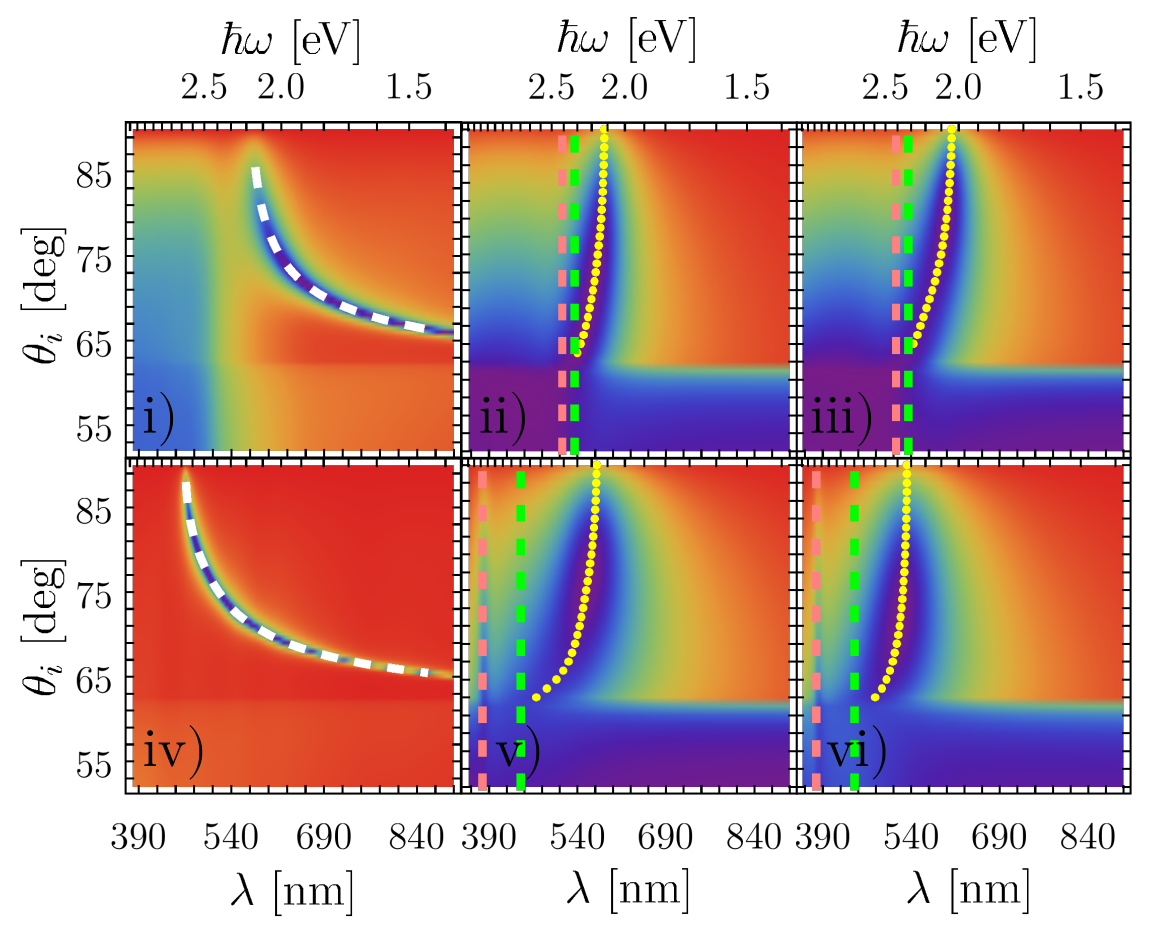
\includegraphics[width =.705\linewidth]{2-Resultados/figs/11-SPPCSM/3-2D_Grid.png}};
\node[right, inner sep=0pt] (legend) at (5.6,.05) {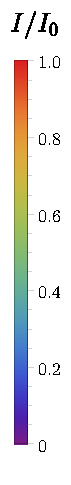
\includegraphics[scale=.96, trim={00 00 00 00}, clip]{2-Resultados/figs/0-IBar_v}};
\node[above, inner sep=0pt] (r) at (5.9,3.75) { $R$};
\end{tikzpicture}
\caption{Gráficas de reflectancia $R$ en configuración ATR, considerando un sustrato con $n_m=1.5$ y una matriz acuosa $n=1.33$, como función del ángulo de incidencia $\theta_i$ y de la longitud de onda $\lambda$ (escala inferior) así como de la energía en unidades de $\hbar\omega$ (escala superior), para una película delgada de $45$ nm de grosor (columna izquierda), y una monocapa de NPs esféricas iluminada por una onda plana en polarización \emph{p} (columna central) y en polarización \emph{s} (columna derecha); los paneles superiores corresponden a una película y NPs de oro con $a=30$ nm y $\Theta=0.125$, mientras que para los inferiores corresponden a una película y NPs de plata de con $a=40$ nm y $\Theta=0.1$.  Las líneas punteadas blancas (columna izquierda) corresponde a los mínimos en la reflectancia debido a la excitación del SPP y lo puntos amarillos (columna central y columna derecha) corresponden a los mínimos en $R$ causados por el modo colectivo predicho por el CSM. Las líneas verticales punteadas verdes corresponden a la SP-SPRs dipolar ($531$ nm y $444$ nm para las NPs empleadas de oro y plata, respectivamente), y las rosas a la SP-SPR cuadrupolar ($514$ nm y $383$ nm para las NPs de oro y de plata, respectivamente).}
\label{fig:SPPCSM}
\end{figure}






\begin{figure}[h!]\centering
\begin{subfigure}{.01\linewidth}\caption{}\label{sfig:R-RVar-cutp}\vspace{4.5cm}\end{subfigure}
	\begin{subfigure}{.45\linewidth}\hspace*{-1.5em}
	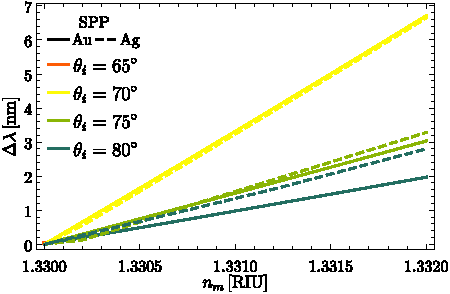
\includegraphics[scale=1]{2-Resultados/figs/11-SPPCSM/4_Sens_h20-SPP.pdf}\end{subfigure}\\
\hspace*{-1.5em}
	\begin{subfigure}{.01\linewidth}\caption{}\label{sfig:R-RVar-cutp}\vspace{4.5cm}\end{subfigure}
	\begin{subfigure}{.45\linewidth}\hspace*{-1.5em}
	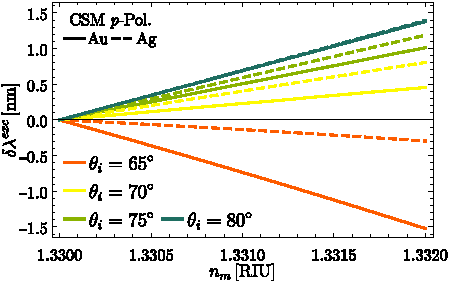
\includegraphics[scale=1]{2-Resultados/figs/11-SPPCSM/5_Sens_h20_CSMP.pdf}\end{subfigure}
	\begin{subfigure}{.01\linewidth}\caption{}\label{sfig:R-RVar-cuts}\vspace{4.5cm}\end{subfigure}\hspace*{-1.em}
	\begin{subfigure}{.45\linewidth}\centering
	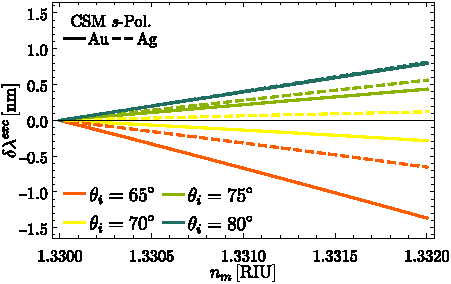
\includegraphics[scale=1]{2-Resultados/figs/11-SPPCSM/6_Sens_h20_CSMS.pdf}\end{subfigure}\vspace*{-.5em}
	\caption{Cortes de la Fig. \ref{fig:R-RVar} a $\theta_i = 75^\circ$ de las gráficas de reflectancia de una monocapa en configuración ATR (Fig. \ref{fig:R-RVar}) de NPs esféricas de fracción de cubierta $\Theta = 0.3$ en polarización \textbf{a)} \emph{p} y \textbf{b)} \emph{s} en función de la longitud de onda $\lambda$ (escala inferior) y de la energía $\hbar\omega$ (escala superior). Los parámetros de la función dieléctrica tipo Drude para las NPs son $\hbar\omega_p = 4.3$ eV y $\hbar\gamma = 0.15$ eV y las fracciones de cubierta consideradas fueron $a$: $3$ nm, $5$ nm, $10$ nm y $20$ nm. La SP-SPR dipolar para los tamaños de partículas utilizadas corresponde la región verde entre $500$ nm y $512$ nm, mientras que la cuadrupolar corresponde a la región rosa entre $456$ nm y $561$ nm.}\label{fig:R-RVar-Cuts}
	\end{figure}	

























